\section{Použité metatechnologie}

\subsection{Git}
\label{subsec:git}

\begin{wrapfigure}{R}{.5\textwidth}
 \centering
 \includesvg[width=.5\textwidth]{assets/git-logo}
 \caption{Logo verzovacího systému Git}
\end{wrapfigure}

Git je distribuovaný systém správy verzí, původně určený pro vývoj jádra Linuxu. Jako jeho autor je označován Linus Torvalds, jeho vznik se datuje kolem 2005 a v~roce 2016 je nadále aktivně vyvíjen; jeho poslední verze nese označení 2.7.3 a byla vydána 10. března 2016. Nejčastěji slouží k~verzování zdrojového kódu - vytváří historii pro každou část spravovaného repozitáře.

Repozitář je v~tomto systému základní nejvyšší jednotka pro správu zdrojového kódu, zapouzdřuje jednotlivé vývojové větvě, ve kterých může probíhat vývoj od jednotlivých vývojářů zcela odděleně. Git je oproti jiným verzovacím nástrojům velmi silný v~následném spojování těchto větví - v~případě nekonfliktních změn je toto spojení schopen provést zcela sám, v~případě těch konfliktních zvládne označit konfliktní místa - pro následné vyřešení konfliktů stačí vyřešit konflikty přímo ve zdrojových souborech, avšak existují i grafická rozhraní. Schéma základních operací je možno pochopit z~obrázku\fullref{fig:git-operations}.

\begin{figure}[H]
 	\centering
 	\includesvg[width=.9\textwidth]{assets/git-operations}
 	\caption{Základní operace při práci se systémem Git}
 	\label{fig:git-operations}
\end{figure}

Git je plně ovladatelný z~příkazové řádky, avšak existuje velké množství jeho grafických nadstaveb, například jednoduchý \href{http://git-cola.github.io/}{git-cola} (náhled v~obrázku\fullref{fig:git-cola}) nebo o~mnoho komplexnější \href{https://www.sourcetreeapp.com/}{SourceTree}.

\begin{figure}[bht]
	\centering
	% \begin{minipage}{.475\textwidth}
 % 		\centering
 % 		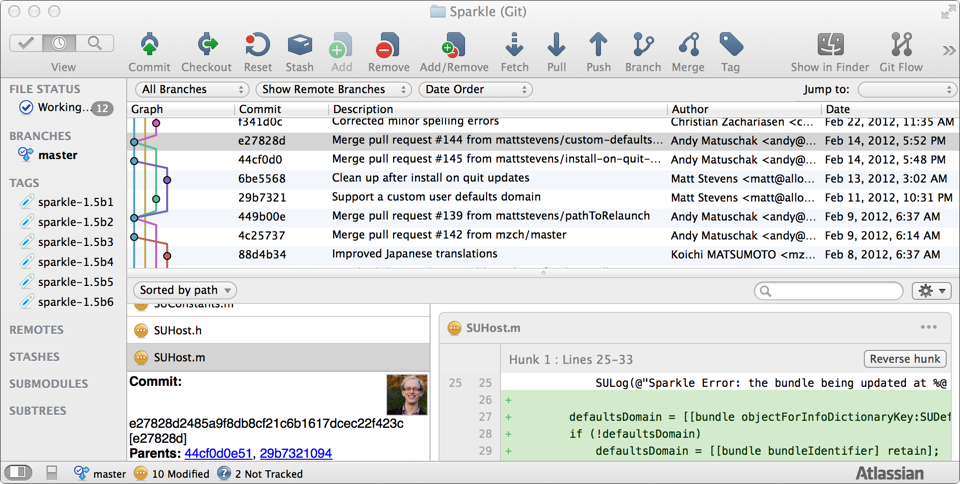
\includegraphics[width=\textwidth]{assets/source-tree-screenshot}
 % 		\caption{Screenshot z programu SourceTree}
	% \end{minipage}
	\begin{minipage}{\textwidth}
 		\centering
 		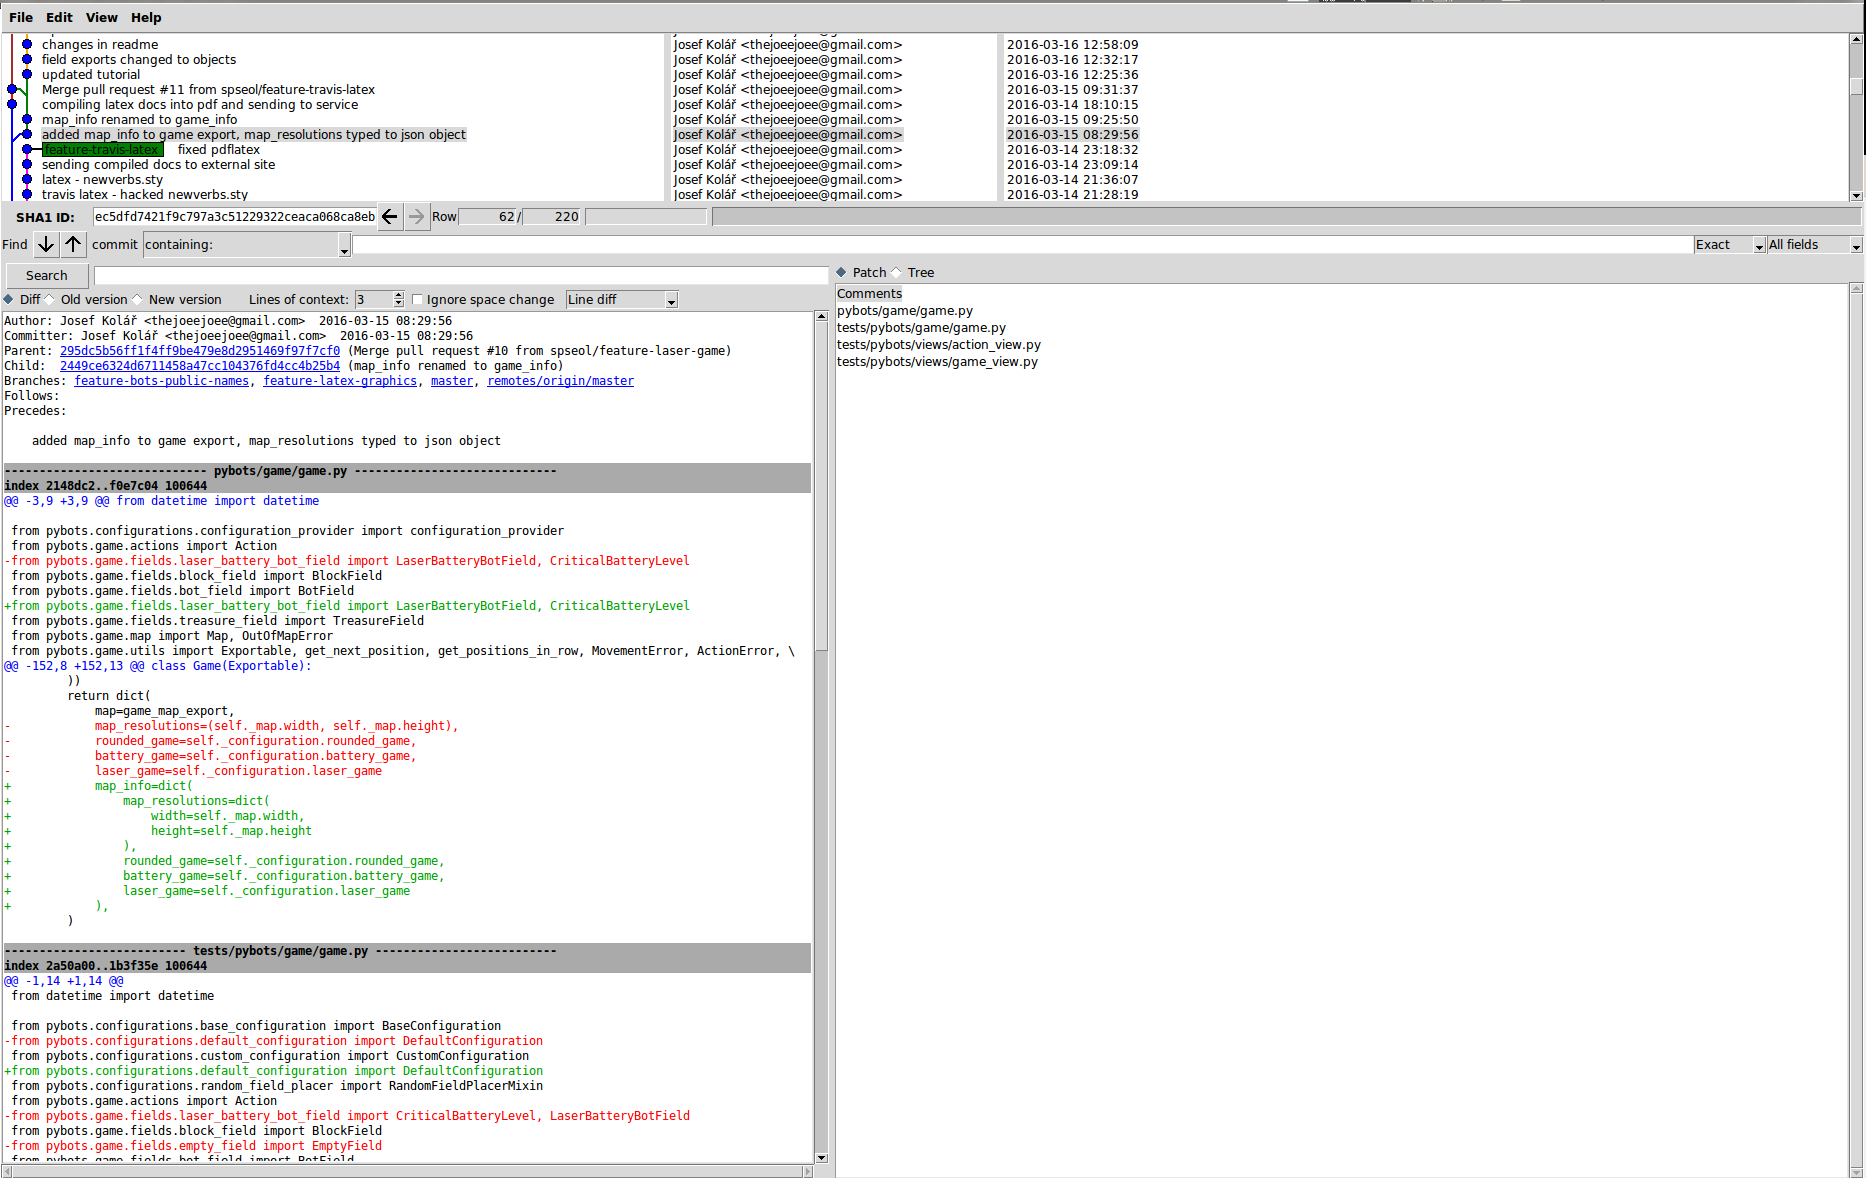
\includegraphics[width=\textwidth]{assets/git-cola-screenshot}
 		\caption{Screenshot z~programu git-cola}
 		\label{fig:git-cola}
 	\end{minipage}
\end{figure}

\subsection{Github}

Github je webová služba poskytující podporu pro hostování \nameref{subsec:git} repozitářů. Pro veřejné repozitáře je tato služba zcela zdarma, pro soukromé repozitáře je zpoplatněna. Kromě hostování nabízí i širokou škálu služeb týkajících se zdrojového kódu, jako například komentování zdrojového k\'{o}du, komentování jeho změn, systém úkolů, soukromých zpráv mezi vývojáři nebo možnost zařazení repozitáře mezi oblíbené. Github spustili v~roce 2008 vývojáři Tom Preston-Werner, Chris Wanstrath a PJ Hyett.

\begin{figure}[bht]
 	\centering
 	\includesvg{assets/github-logo}
 	\caption{Logo systému pro správu git repozitářů GitHub}
\end{figure}

\subsection{Travis CI}

\begin{figure}[bht]
	\centering
	\includesvg{assets/travis-logo}
	\caption{Logo automatického buildovacího nástroje Travis CI}
\end{figure}

\todo{popsat Travis-CI}

\subsection{Pycharm}

\begin{figure}[bht]
	\centering
	\includesvg{assets/pycharm-logo}
	\caption{Logo vývojového nástroje Pycharm}
\end{figure}

\todo{popsat Pycharm}